
%(BEGIN_QUESTION)
% Copyright 2010, Tony R. Kuphaldt, released under the Creative Commons Attribution License (v 1.0)
% This means you may do almost anything with this work of mine, so long as you give me proper credit

A form of liquid level switch called a {\it tilt switch} is often used for detecting sewage level in ``lift stations'' where sewage collected from homes via gravity is pumped out of the collection sump to the wastewater treatment plant (usually located miles away):

$$\includegraphics[width=15.5cm]{i00037x01.eps}$$

Suppose the pump motor refuses to start even with the sump level above the LSH position:

$$\includegraphics[width=15.5cm]{i00037x02.eps}$$

An electrician claims this could be the result of the M1 auxiliary contact (connected in parallel with the LSH) being failed open.  Do you agree?  Also, identify at least two other possible causes of the pump not starting at a high-level condition.

\vfil 

\underbar{file i00037}
\eject
%(END_QUESTION)





%(BEGIN_ANSWER)

This is a graded question -- no answers or hints given!

%(END_ANSWER)





%(BEGIN_NOTES)

A failed-open M1 auxiliary contact would account for the pump not {\it latching} (i.e. not remaining on after the liquid level falls below the LSH point), but it would not explain why the motor fails to start in the first place.

\vskip 10pt

Other possible faults include:

\begin{itemize}
\item{} Failed-open OL contact
\item{} Failed-open LSH switch
\item{} Failed-open LSL switch
\item{} 120 VAC control power off (L1/L2)
\item{} Failed-open contactor coil M1
\item{} Failed-open power contacts (M1 in three-phase circuit)
\item{} Failed-open motor windings
\end{itemize}

%INDEX% Measurement, level: switch
%INDEX% Process: wastewater lift station
%INDEX% Troubleshooting review: electric circuits

%(END_NOTES)


